\documentclass[onecolumn, draftclsnofoot,10pt, compsoc]{IEEEtran}
\usepackage{graphicx}
\usepackage{url}
\usepackage{setspace}
\usepackage{listings}
\usepackage[center]{caption}
\usepackage{float}
\usepackage{pgfgantt}

\usepackage{geometry}
\geometry{textheight=9.5in, textwidth=7in}

% 1. Fill in these details
\def \CapstoneTeamName{The Cleverly Named Team}
\def \CapstoneTeamNumber{40}
\def \GroupMemberOne{Brian Hambleton}
\def \GroupMemberTwo{Dakota Alton}
\def \GroupMemberThree{Ian Band}
\def \GroupMemberFour{Ivan Halim}
\def \CapstoneProjectName{Converting Fortran to Python}
\def \CapstoneSponsorPerson{Genevieve Segol}

% 2. Uncomment the appropriate line below so that the document type works
\def \DocType{Winter Term Progress Report}
			
\newcommand{\NameSigPair}[1]{\par
\makebox[2.75in][r]{#1} \hfil 	\makebox[3.25in]{\makebox[2.25in]{\hrulefill} \hfill		\makebox[.75in]{\hrulefill}}
\par\vspace{-12pt} \textit{\tiny\noindent
\makebox[2.75in]{} \hfil		\makebox[3.25in]{\makebox[2.25in][r]{Signature} \hfill	\makebox[.75in][r]{Date}}}}
% 3. If the document is not to be signed, uncomment the RENEWcommand below
\renewcommand{\NameSigPair}[1]{#1}

%%%%%%%%%%%%%%%%%%%%%%%%%%%%%%%%%%%%%%%
\begin{document}
\begin{titlepage}
    \pagenumbering{gobble}
    \begin{singlespace}
        \hfill 
        \par\vspace{.2in}
        \centering
        \scshape{
            \huge CS Capstone \DocType \par
            {\large\today}\par
            \vspace{.5in}
            \textbf{\Huge\CapstoneProjectName}\par
            \vfill
            {\large Prepared for}\par
            {\Huge\NameSigPair{\CapstoneSponsorPerson}\par}
            {\large Prepared by }\par
            Group\CapstoneTeamNumber\par
            % 5. comment out the line below this one if you do not wish to name your team
            % \CapstoneTeamName\par 
            \vspace{5pt}
            {\Large
                \NameSigPair{\GroupMemberOne}\par
                \NameSigPair{\GroupMemberTwo}\par
                \NameSigPair{\GroupMemberThree}\par
                \NameSigPair{\GroupMemberFour}\par
            }
            \vspace{20pt}
        }
        \begin{abstract}  
        This document is an overview of work completed, tasks left to be completed and problems encountered from January 7th to March 15th.
        \end{abstract}     
    \end{singlespace}
\end{titlepage}
\newpage
\pagenumbering{arabic}
\tableofcontents
% 7. uncomment this (if applicable). Consider adding a page break.
%\listoffigures
%\listoftables
\clearpage
\section{Project Recap}
Specialized software used in research is often found to be outdated due to its complexity and the limited number of people with expertise on the relevant subject who are also able to maintain the software. This can cause such programs, written in older languages, to lose support over time and become unusable by researchers. The purpose of this capstone project is to modernize one such piece of software to make it more readily available and accessible for researchers. The software in question, originally written in Fortran, preforms analysis of flow and mass transport in unsaturated, partially saturated and fully saturated flow regions to be used for the evaluation of  sites for waste disposal. The software would still be useful today if it were accessible to researchers, however, the mainframes that the original program was written for are no longer in use. The software in its current state must be modernized in order to be useful.
\\\\
The goals of the project are as follows:
\begin{itemize}
    \item Produce an updated version of the code that can be run on modern consumer hardware with minimal setup required.
    \item Increase the ease of data input to the program.
    \item Rewrite the data visualization portion of the project with modern graphics tools in Python 3. 
\end{itemize} 
\section{Where We Stand}
We have achieved beta functionality for each of the previously specified goals. We have a version of the original Fortran code, ported to C, that can be run on modern systems. We have created a GUI that allows users to setup their scenario through manual input or via file upload. The parameters are then saved to data files to be read by the simulation. Lastly, we have a section of the GUI meant for visualizing the state of the mesh being evaluated in the simulation.\\\\
The updated version of the simulation, written in C, is capable of being run as a standalone application, but it can also be run from within the GUI we have developed. Calling it from the GUI is the primary method for running the simulation.\\\\
The GUI we have created has inputs for all fields required by the simulation. Additionally, it has sections for users to preview the initial state of the mesh being evaluated as well as a section for viewing the output of the simulation as text.

\section{What Remains}
There are two remaining tasks to complete before the spring expo. We need to debug the simulation and we need to add callbacks to the main loop of the simulation that will allow us to view the mesh throughout the simulation's run time.\\\\
We suspect that the primary bug with our port of the simulation has to do with creating the cubic splines used to interpolate values. We are working on narrowing down the issue, but are fairly confident that we will be able to resolve the issue. \\\\
As for getting run time updates on the mesh, we have a robust system in the C code that will give the GUI a copy of the mesh being evaluated. So seeing the mesh change through run time will be a matter of utilizing this system at the correct times. Accomplishing this task will pretty much fallout of debugging the simulation. 

\section{Problems Encountered}
The main issue we encountered with our design had to do with the version of Fortran used to write the original program. Our initial research into how we might solve the problem lead us to a tool known as F2PY which supports interfacing with Fortran 77 code. This tool should have been able to convert the original Fortran code into an intermediary format which would have allowed us to call the Fortran code from Python. This option did not pan out as it was determined the original code was written in Fortran IV (66), not Fortran 77 as the original program's documentation states, which is not supported by F2PY.\\\\
We overcame this issue by porting the Fortran code to C and wrapping the resulting C library in Python. There are three reasons for porting to C. First, speed gains are not lost when calling C from Python. Second, parameters to subroutines in Fortran are all by reference, meaning the subroutine can modify them and the change can be seen outside of the subroutine. C allows for this behavior where Python doesn't without writing hacky code. The third reason is that the GNU foundation offers a C library called GSL which we were able to use to mimic the functionality of the IMSL library used by the fortran code. 
\section{Screenshots}
\begin{figure}[H]
    \centering
    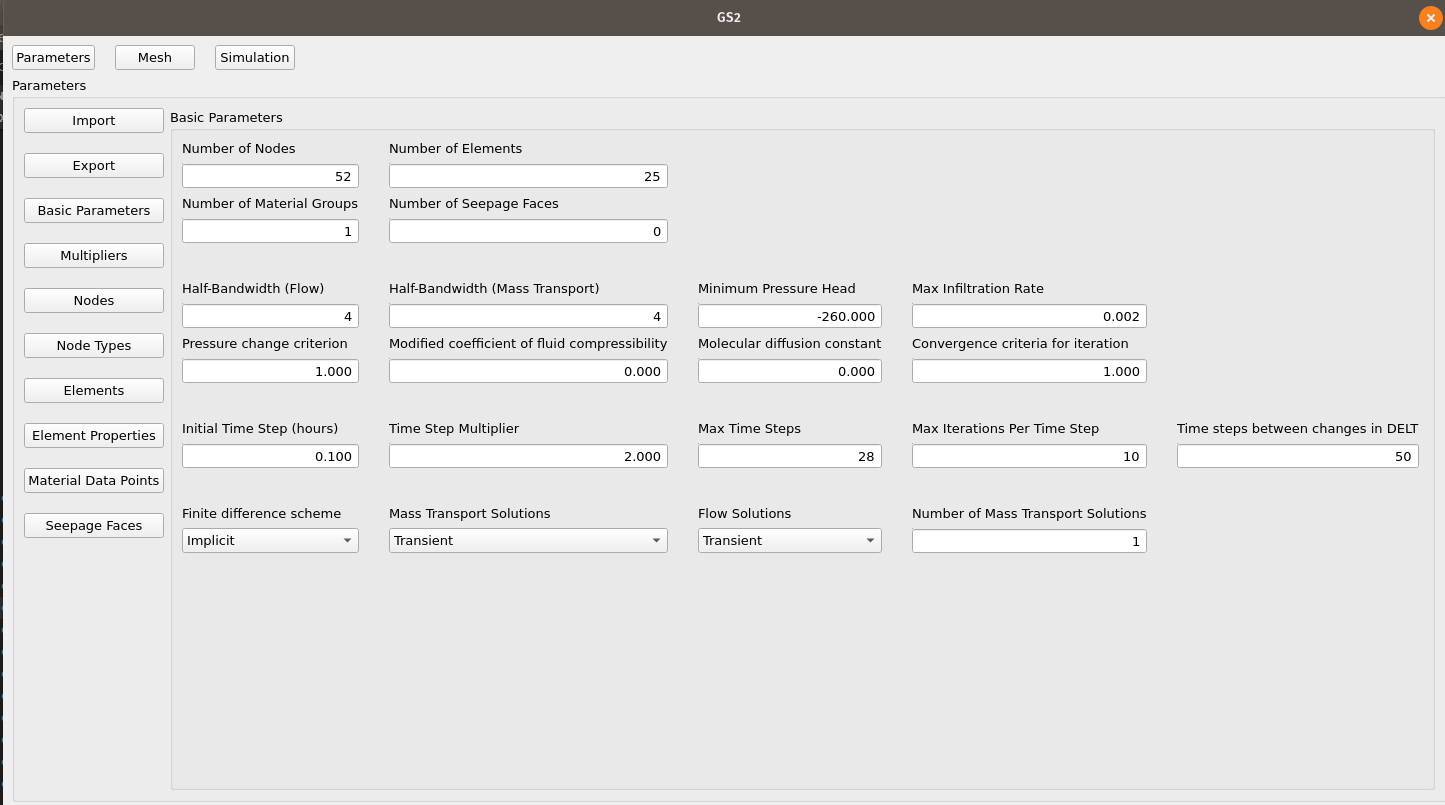
\includegraphics[scale=0.3]{basic-parameters.png}
    \caption{Basic Parameters Screen}
    \label{fig:basic-parameters}
\end{figure}{}
Figure \ref{fig:basic-parameters} shows the screen a user is met with when they first launch the application. This screen allows the user to input data that dictates how the simulation will run. That is it defines meta data for the simulation. 
\begin{figure}[H]
    \centering
    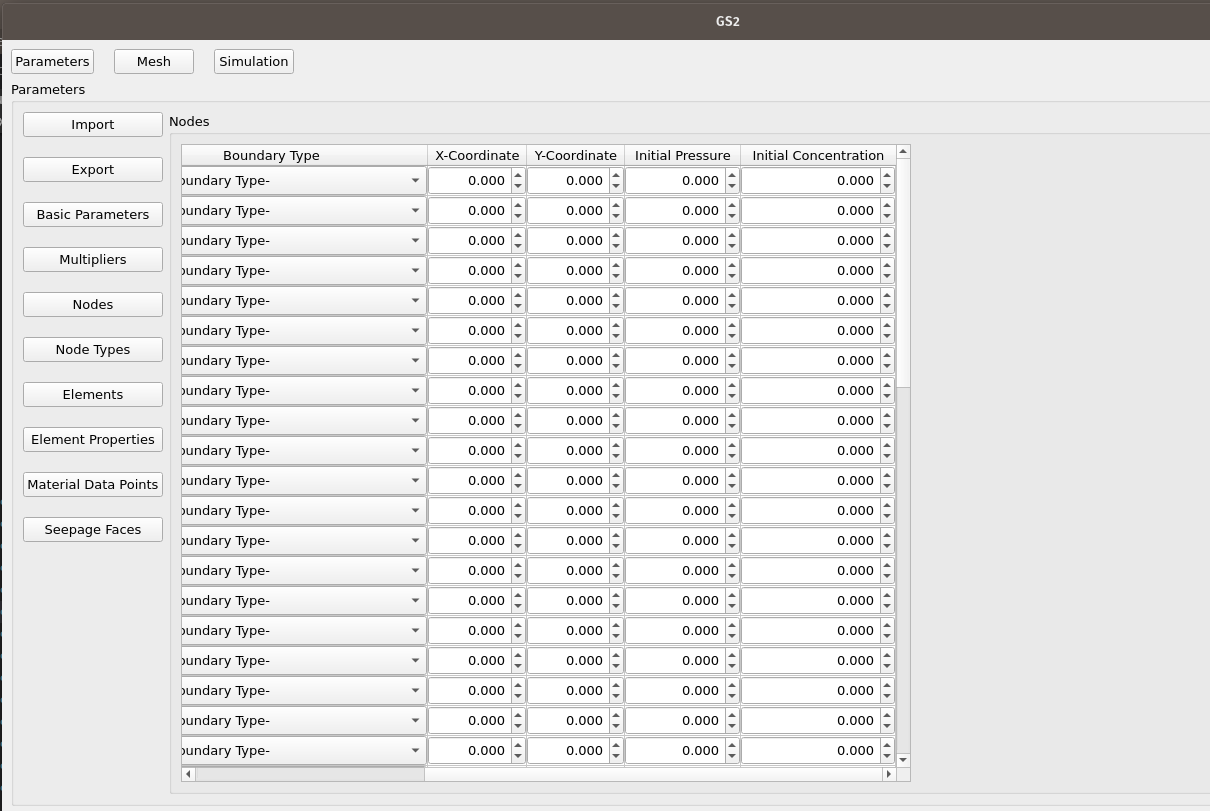
\includegraphics[scale=0.3]{node-data.png}
    \caption{Node Data Screen}
    \label{fig:node-data}
\end{figure}{}
Figure \ref{fig:node-data} shows a table that lets the user input data for nodes that model the transport problem being simulated. 
\begin{figure}[H]
    \centering
    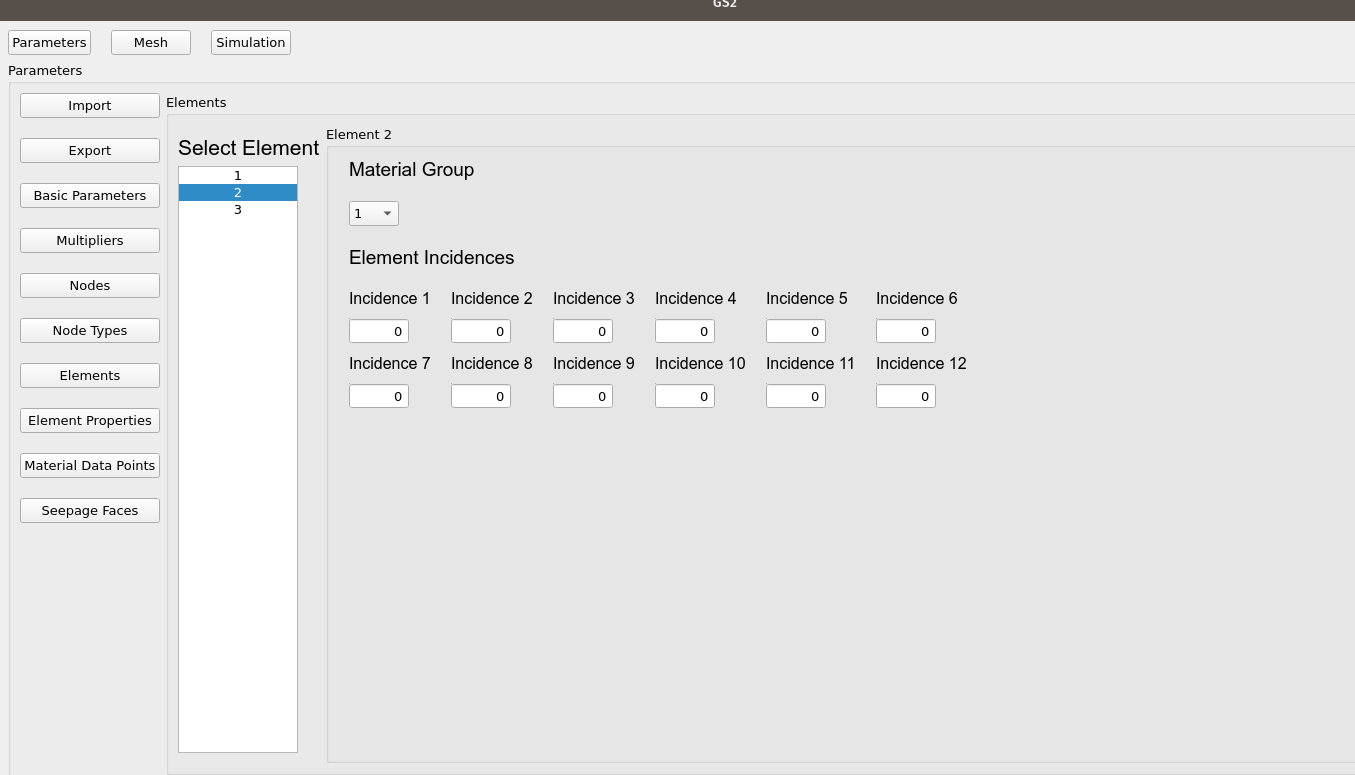
\includegraphics[scale=0.3]{element-incidence.png}
    \caption{Element Incidence Screen}
    \label{fig:element-incidence}
\end{figure}{}
Figure \ref{fig:element-incidence} shows the screen where a user can specify elements in the model. These elements have different properties that affects how analysis is done in different sections of the model. 
\begin{figure}[H]
    \centering
    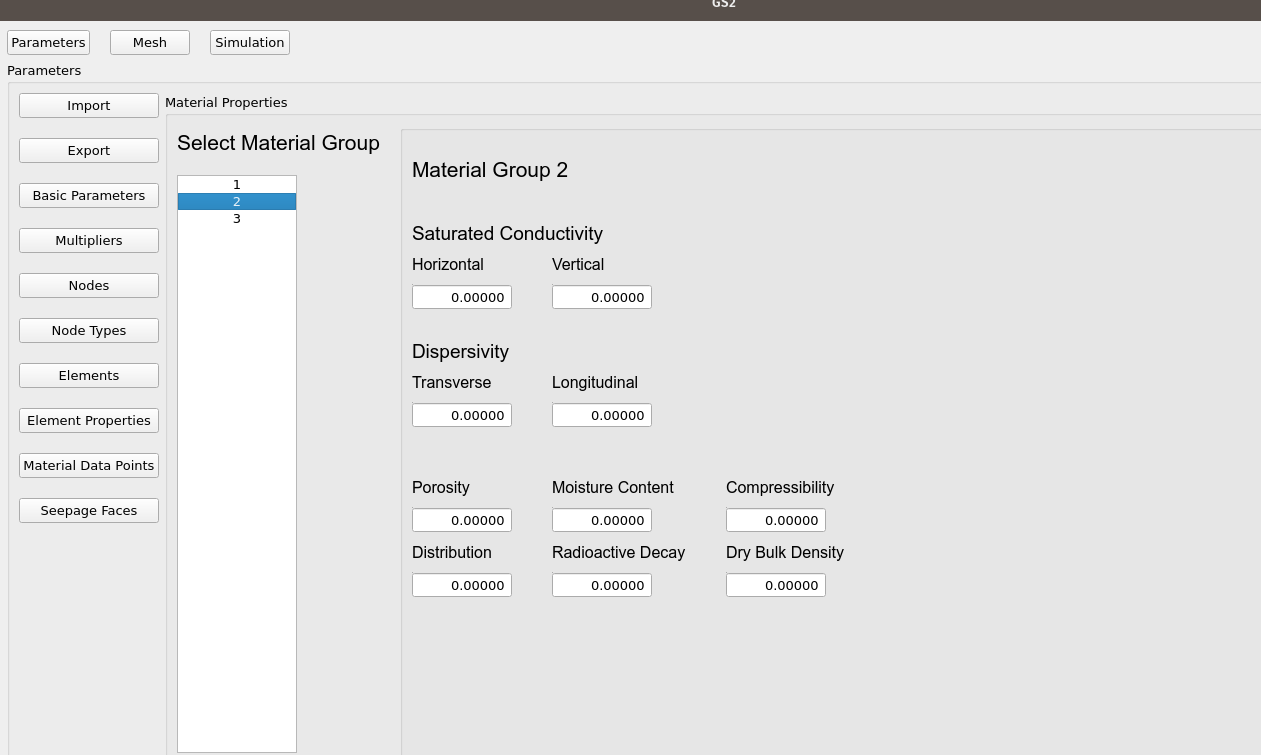
\includegraphics[scale=0.3]{element-properties.png}
    \caption{Element Material Properties}
    \label{fig:element-properties}
\end{figure}{}
Figure \ref{fig:element-properties} shows the screen where a user can specify material group properties for different elements. 
\begin{figure}[H]
    \centering
    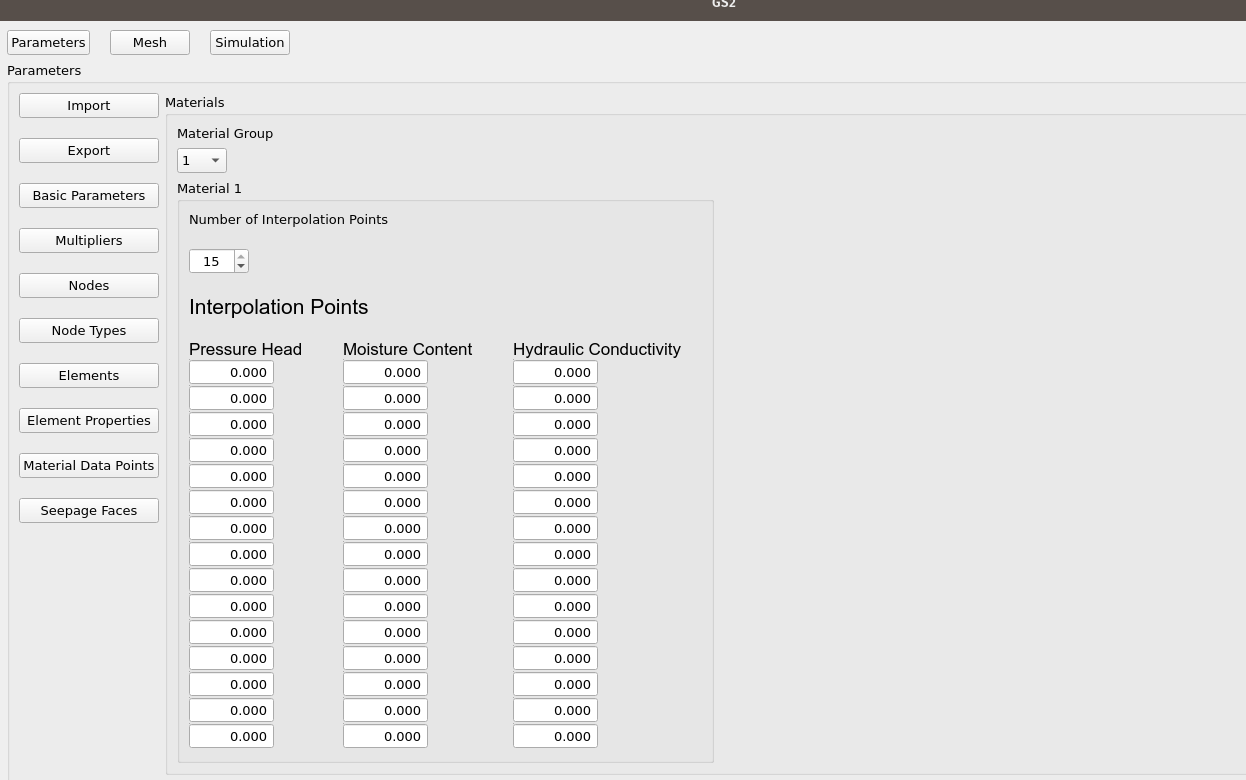
\includegraphics[scale=0.3]{material-properties.png}
    \caption{Material Properties Screen}
    \label{fig:material-properties}
\end{figure}{}
Figure \ref{fig:material-properties} shows the screen where a user can specify material properties. 
\begin{figure}[H]
    \centering
    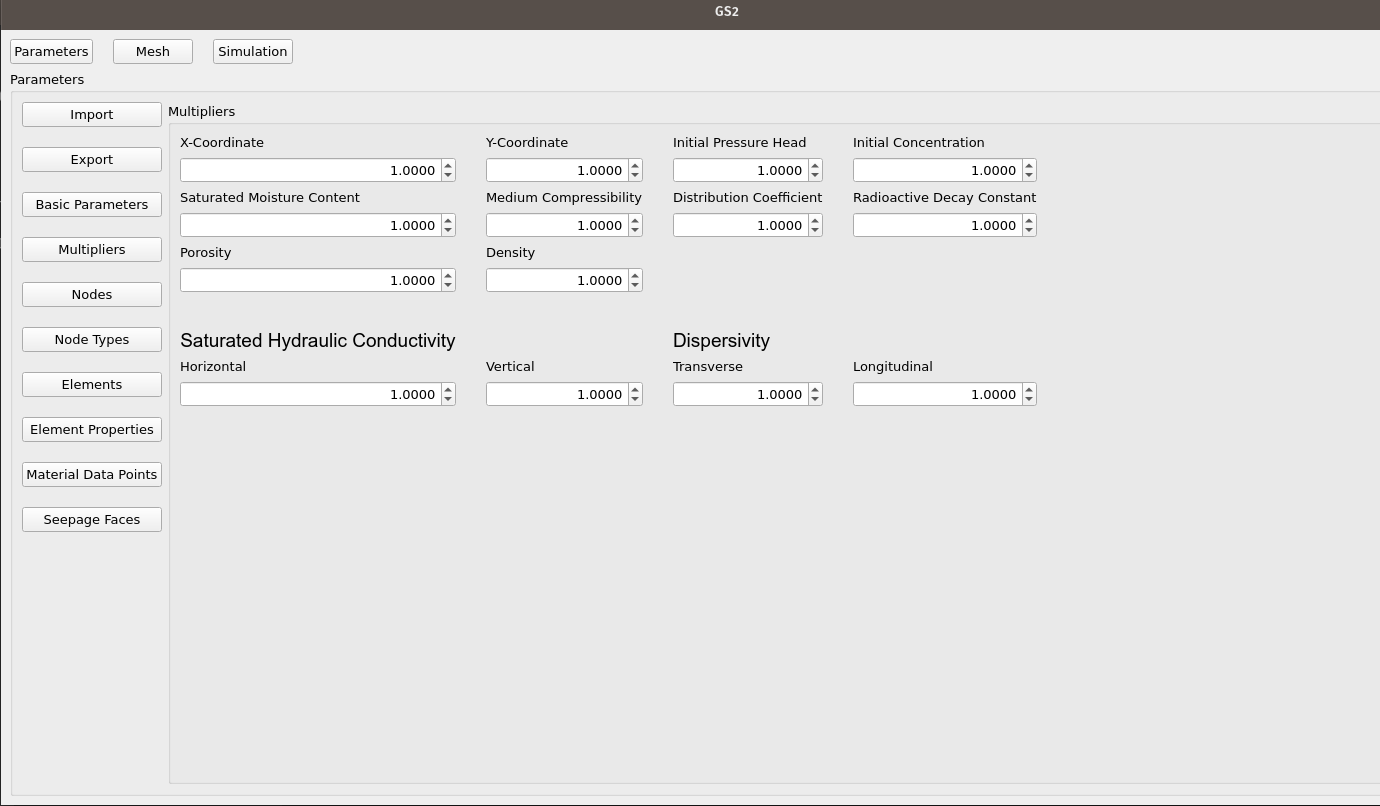
\includegraphics[scale=0.3]{multipliers-scree.png}
    \caption{Multipliers Screen}
    \label{fig:multipliers}
\end{figure}{}
Figure \ref{fig:multipliers} shows the screen where the user can input multipliers for the simulation. These values affect how data is processed in the simulation. 
\begin{figure}[H]
    \centering
    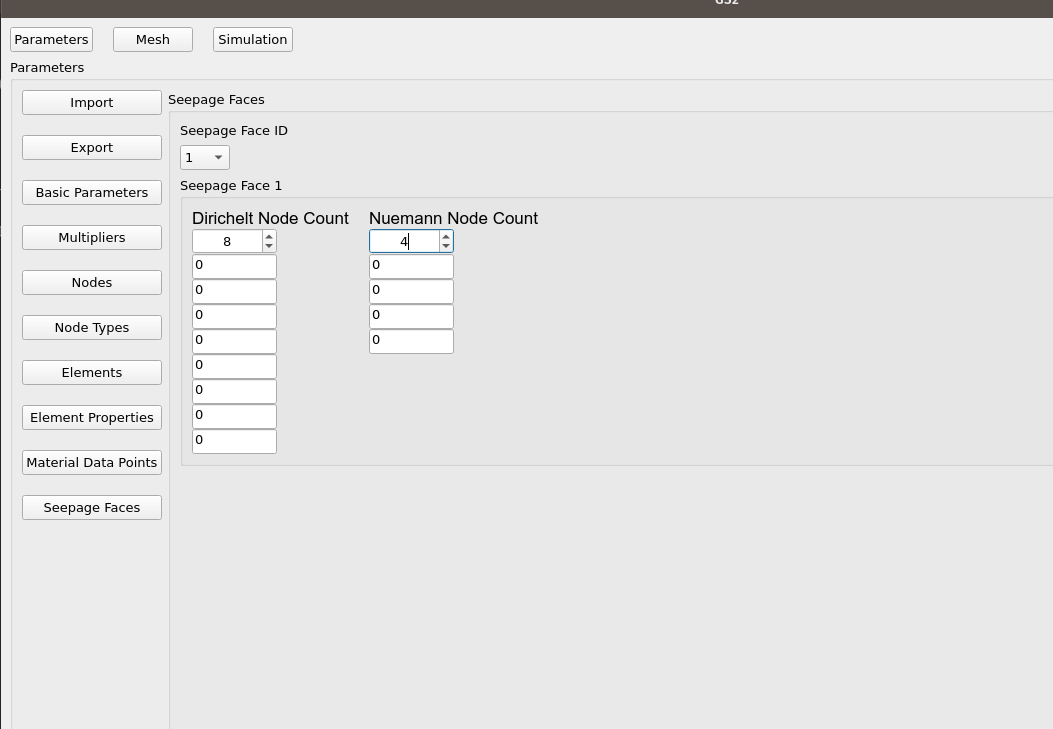
\includegraphics[scale=0.3]{seepage-face.png}
    \caption{Seepage Face Screen}
    \label{fig:seepage-face}
\end{figure}{}
Figure \ref{fig:seepage-face} shows the screen that allows the user to specify seepage faces for the model. Seepage faces affect how integration is computed. 
\begin{figure}[H]
    \centering
    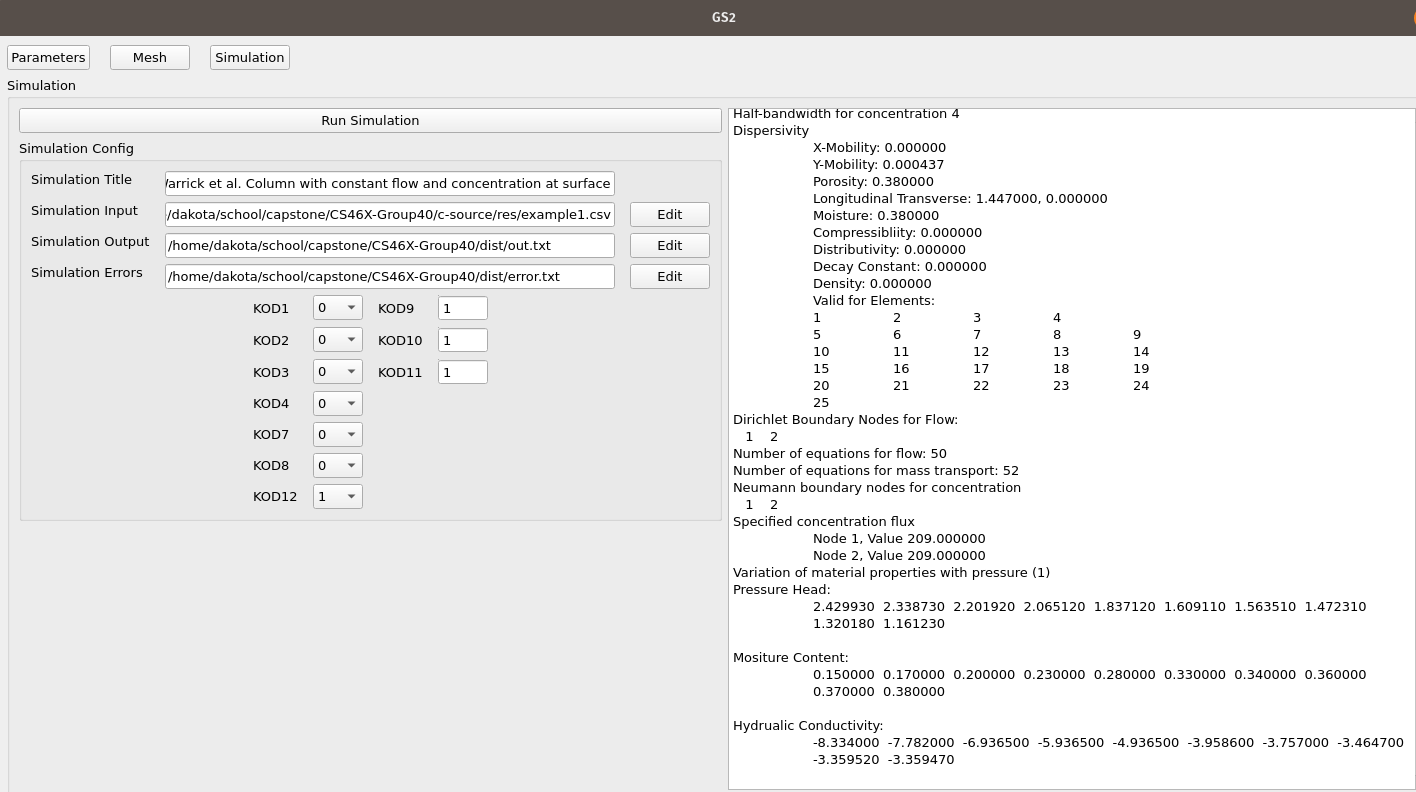
\includegraphics[scale=0.3]{run-sim-page.png}
    \caption{Run Simulation Screen}
    \label{fig:run-sim}
\end{figure}{}
Figure \ref{fig:run-sim} allows the user to run the simulation. Additionally it has inputs that allows the user to control IO for the simulation. That is, from this screen the user can decide which data file to read into the simulation, where the output should be written, and where the simulation should log errors to.
\begin{figure}[H]
    \centering
    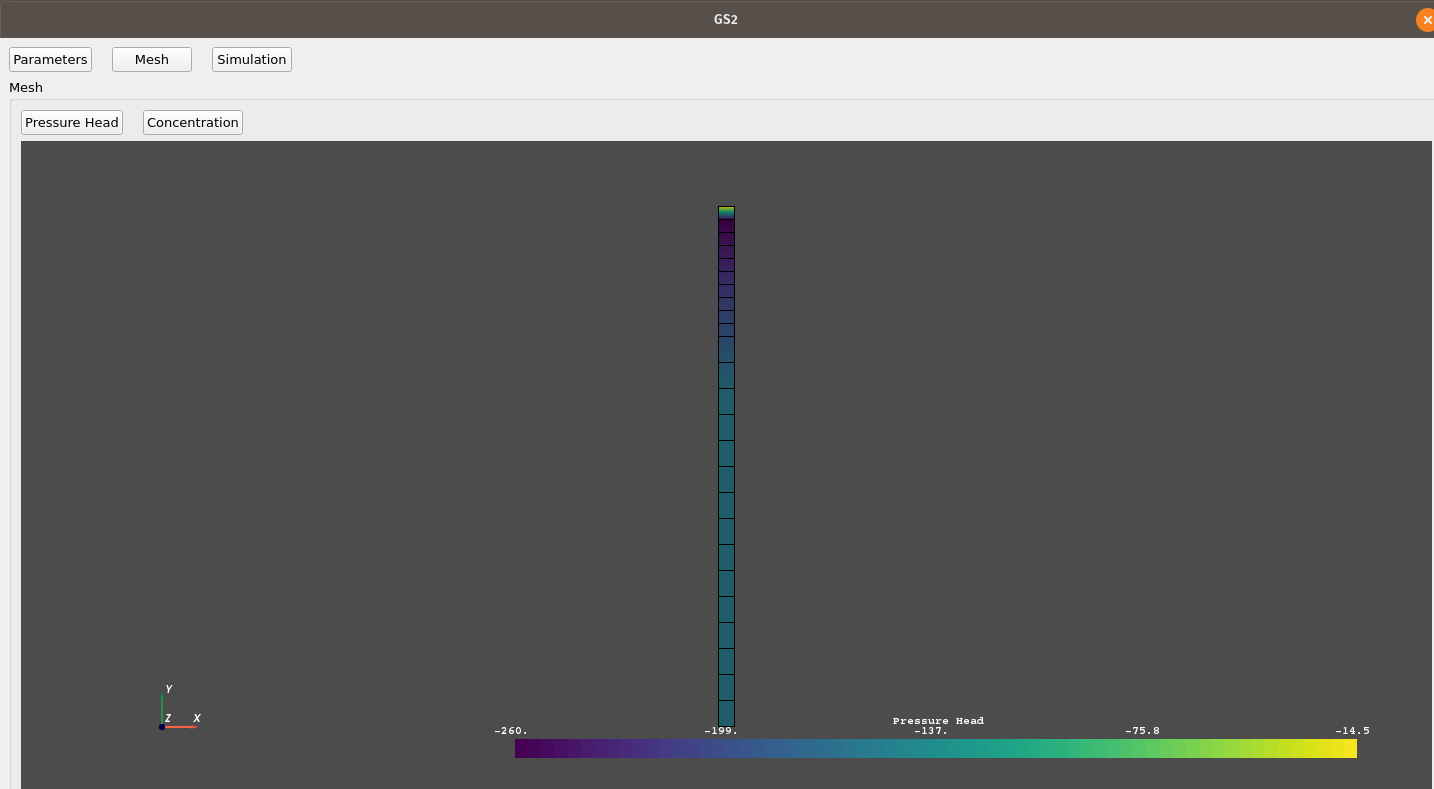
\includegraphics[scale=0.3]{mesh-screen.png}
    \caption{Mesh Viewing Screen}
    \label{fig:mesh-screen}
\end{figure}{}
Figure \ref{fig:mesh-screen} shows the mesh of the model that the simulation is evaluating. In our applications current state, the mesh shown represents the initial state of the model.
\end{document}
